\subsection{Handbuch}
\subsubsection{Aufgaben}
Das Handbuch ist wesentlicher Bestandteil der Software und soll sowohl die Funktionsweise der einzelnen Komponenten als auch deren Verwendung erklären. Grundsätzlich enthält das Handbuch den Großteil dieser schriftlichen Ausarbeitung, da auch hier auf die Funktionsweise der einzelnen Teilbereiche eingegangen wird. 

\subsubsection{Aufbau}
In der Anwendung wird das Handbuch als eigener Tab angezeigt da es um den Anforderungen einer Schulungssoftware gerecht zu werden als eine der Hauptfunktionen der Anwendung gesehen wird. Wählt ein Benutzer den Entsprechenden Tab "Handbuch" aus, so bekommt er im Hauptfenster der Anwendung das Handbuch angezeigt. 
Die Navigation innerhalb des Handbuches ist hierbei über eine Baumstruktur realisiert und basiert auf der Auflistung einzelner Kapitel und Unterkapitel.

\subsubsection{Bedienung der Oberfläche}
\begin{figure}[H]
  \centering
  \begin{minipage}[t]{12 cm}
  	\centering
  	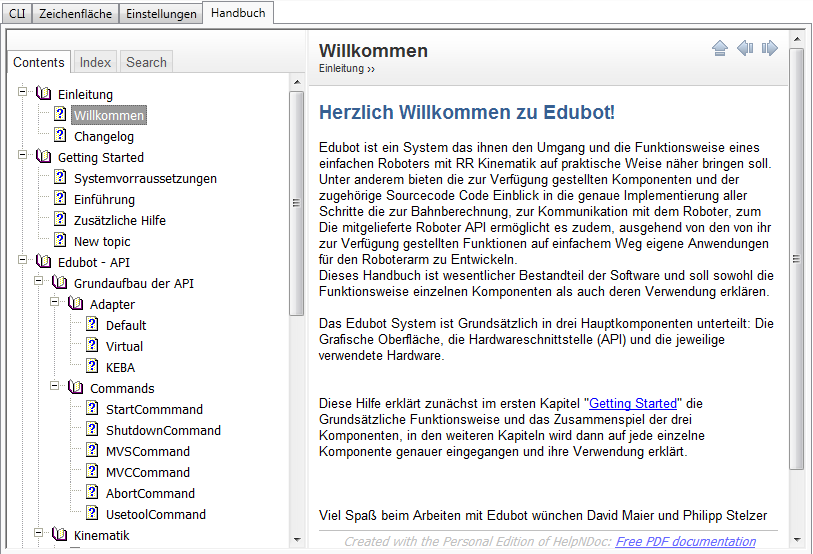
\includegraphics[width=12cm]{images/Manual} 
    \caption{Das Handbuch}
  \end{minipage}
\end{figure}
Die Bedienung des Handbuchs sollte selbstverständlich sein. Auf der linken Seite befindet sich ein Baum mit den entsprechenden Kapiteln. Wenn auf ein Kapitel geklickt wird dessen Inhalt angezeigt.

\subsubsection{Umsetzung}
Geschrieben wurde das Handbuch mit Hilfe der Anwendung HelpNDoc, auf welche in dieser schriftlichen Arbeit bereits eingegangen wurde. Durch den Export als HTML Datei bietet sich die Möglichkeit das Handbuch über das von WPF zur Verfügung gestellte Controll \textit{WebBrowser} einfach in die Anwendung einzubinden. 

Hierzu muss lediglich ein neues \textit{WebBrowser} Controll im Entsprechenden Tab erzeugt und im Programmcode der Aufruf der entsprechenden HTML Datei konfiguriert werden.
Wichtig ist hierbei, dass dieser Aufruf nicht über den absoluten lokalen Pfad, sondern über die Loopback IP des PC's (127.0.0.1) geschieht, da sonst die benötigten ActiveX bestandteile des Handbuches gesperrt werden.